If there is a predictive theory, as the Higgs field in the Standard Model for any given (but a priori unknown) Higgs boson mass, the rate of events will predict that a statistical analysis should see if the theory is true. This chapter will give a brief review of the analysis techniques used to reconstruct Higgs signal and determine signal strength modifier using the CMS results, and also checks if hypothesis tests are compatible with the statistical techniques.  This will ensure the validity of the data collected for Higgs boson mass and will help in categorizing events which are accumulated in the detector. 
\section{Hypothesis Testing in Research Study}
If the measured event rate in a search is more than the expected event rate, than the Standard Model theory is untrue (i.e. there is no Higgs boson, at least not at that mass). For verification of a theory, the expected event rate and measured event rate should have 99.99994\% coincidence level after background reduction which can be achieved when there is unlimited amount of data.\\
Now we not only see if the new particle (or whatever) is actually there, but also if it is there at a rate in agreement with the prediction of its origin. For that we need to decide that, statistically how close the measured rate is to the predicted one.\\
The “rate” is the one that appears in  Poisson probability as $\lambda$ in $p(k|\lambda)=\lambda^{k} e^{-\lambda}/k!$, this gives the probability of having seen $k$ events, when our theory told us to expect $\lambda$. (This picture is complicated by systematic
uncertainties, which are not perfectly defined, but one with uncertainties of its own). In the direct prediction from the theory, we usually have $\lambda=s+b$, where $s$ is expected rate from the signal process, and $b$ is the expected rate from background processes (assumption: both don’t interfere).
The signal strength modifier is a number, usually denoted by $\mu$ which is multiplied to the standard, predicted signal rate: $\lambda \rightarrow \lambda'=\mu s+b$ . This allows that at 95\% statistical uncertainty and the 125 GeV Higgs boson production rate is between 80\% and 130\% of the Standard Model value, i.e. still statistically
very compatible with the SM.\\
Those bounds would correspond to $\mu=0.8$ and $\mu=1.3$ respectively. Much more exciting would be a limit range that did not include 1; that would imply a deviation from the Standard Model after which codes and systematic constraining methods should be double checked.
Statistics here follow Poisson trends, so if we have a high rate, the statistical uncertainty on assessing that rate will be small and so assuming that various systematic uncertainties have been brought under control we can test the theory in some precision very rapidly, but if the rate is low then its uncertainty will be relatively large and harder to pin down. The more data we take, the better the statistical constraint will be \cite{<quora>}.\\
Note also that likelihood and signal strength are directly connected: values of $\mu$ that take
$\lambda$ closer to the observed rate will get a high likelihood, while those that predict rates far
from the observed can be ruled out. We draw a 2D plot of $\mu$ versus a fixed threshold likelihood of 95\% used above and mark the values of $\mu$ where it’s crossed.
\section{Hypothesis Testing of Higgs Signal}
The search for the $\PHiggs \rightarrow \Pmuon + \APmuon$ signal can be formulated as a hypothesis test. The null or background only hypothesis explains the case where only the known SM backgrounds exist, but no signal is present. The other hypothesis is that the background and the signal we are looking for both exist. The modified frequent method or $CLs$ method \cite{<cls>} is used to quantify which hypotheses are favored or excluded.\\
All hypotheses that are considered in this analysis can be expressed as $\mu s+b$, where $\mu$ is the so called signal strength parameter. The signal with background hypothesis corresponds to $\mu$=1 and $\mu$=0 is for the background hypothesis for a Standard Model Higgs boson decay. To estimate the level of compliance of a hypothesis in question, with the measured data, we propose a test statistic $\PSq_{\mu}$. It is a function containing events (signal and bakgrounds) and the standard parameter, in our case the signal strength $\mu$. It is constructed in such a way that a higher value of $\PSq_{\mu}$ indicates a higher incompatibility amongst the data and the chosen $\mu$-hypothesis.
The p-value, defined as the probability of statistics kept for checking is equal or more than the one observed, for a given hypothesis is then calculated to quantify this disagreement. This is illustrated in Fig.\ref{fig:asym}(a). To calculate a p-value the probability distribution function is integrated over all values of $\PSq_{\mu}\ge\PSq_{\mu,obs}$
\begin{equation}
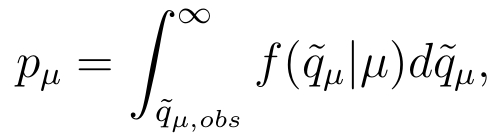
\includegraphics[scale=0.3]{images/1.jpg}
\end{equation}
here $\PSq_{\mu,obs}$ is the number observed from data of the statistics we used for checking and gives the probability distribution function (PDF) of $\PSq_{\mu}$. This PDF has been probed by Monte Carlo pseudo-experiments, where repeatedly Poisson distributions of $m_{\mu\mu}$ according to the hypothesis have to be generated and corresponding test statistic is then computed.\\
For Higgs analysis log-likelihood ratio is used:
\begin{equation}
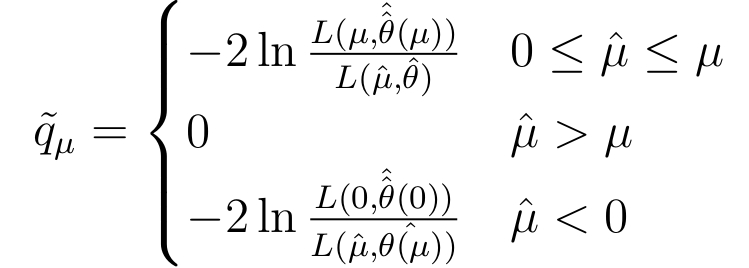
\includegraphics[scale=0.3]{images/2.jpg}
\end{equation}
The likelihood $L$ is based on the best fit of both, signal model and background model put together to the $m_{\mu\mu}$ spectrum. In the formula for the test statistic, $\theta$ are used but are not of interest themselves, the so called nuisance parameter. $\hat{\mu}$ and $\hat{\theta}$ are the best fit values for $\mu$ and $\theta$ floating free in the fit. $\hat{\theta}$ is calculated by a fit with a fixed $\mu$, but floating $\theta$.
In particle physics we commonly change the p-value into an equivalently important $Z$. The local significance of a deviation from the null hypothesis is calculated from $p_{0}$ , the corresponding p-value. It is defined when a standard Gaussian distributed variable, is seen as $Z$ standard deviations more than its mean, with an upper tail probability equivalent to $p$ given as,
\begin{equation}
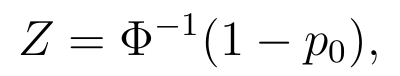
\includegraphics[scale=0.3]{images/3.jpg}
\end{equation}
where the cumulative distribution inverse $\Phi^{-1}$ of a typical Gaussian distribution is illustrated in Fig.\ref{fig:asym}(b). To claim discovery it is customary to gain a reading of at least $Z>5$.
\begin{figure}[h]
\centering
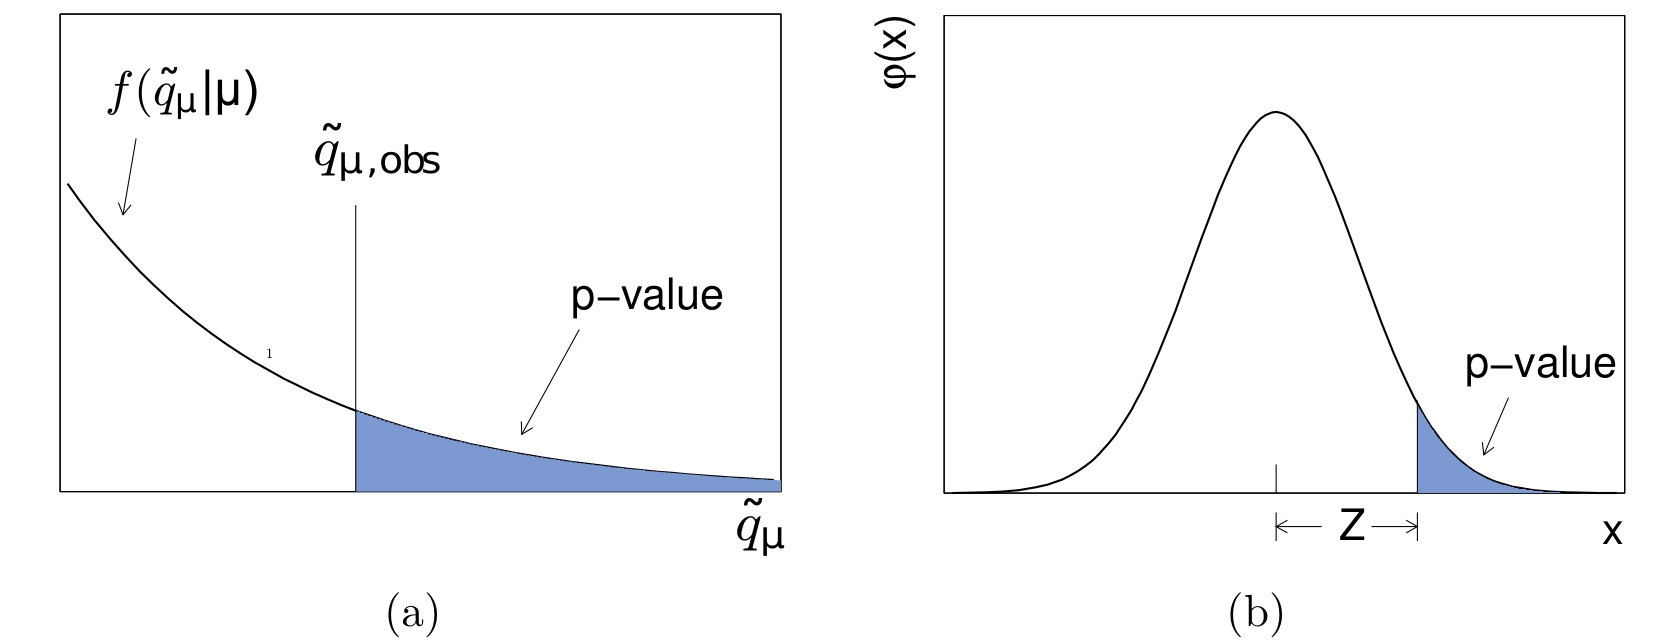
\includegraphics[scale=0.3]{images/4.jpg}
\caption{(a) p-value obtained using a test statistic $\hat{q}_{\mu}$. (b) Relationship between p-value and local significance Z as
derived from a standard Gaussian distribution $\phi(x)$ = $(1/ 2\sqrt{\pi})exp(-x ^{2}/2)$. Images adapted from \cite{<asym>}.}
\label{fig:asym}
\end{figure}
\section{Signal Strength Modifier of Higgs Signal}
Higgs-Signals are defined as the signal strengths at either a given mass peak or as functions of Higgs masses, considered as an observable in a computer code. The preliminary samples accumulated for Higgs-Signals via hadron colliders, are mainly by the LHC experiments, and is supported by the data from Tevatron. The Higgs-Signals methods have far reaching applications, for instance, data collection from a future $\eplus\eminus$ linear collider. 
This section will focus on the description of the experimental data that grants us the basic input for Higgs-Signals \cite{<ss1>}\cite{<ss2>}.\\
Explorations for Higgs bosons in CMS experiment are proceeded with the assumptions made in the Standard Model, such as Higgs-fermion couplings and Higgs-vector boson couplings, and both the cross sections and branching ratios are stated as a function of the Higgs boson mass, $m_{H}$. This gives permission for measuring one-parameter scaling e.g. $1\sigma$ of the total SM rate of a certain signal channel(s), supposedly signal strength modifiers, which come from best fitted data. They represent the basic observable input adopted in Higgs-Signals estimation. Samples from ATLAS and CMS are demonstrated in Fig.\ref{fig:sig1}.\\
\begin{figure}[h]
\centering
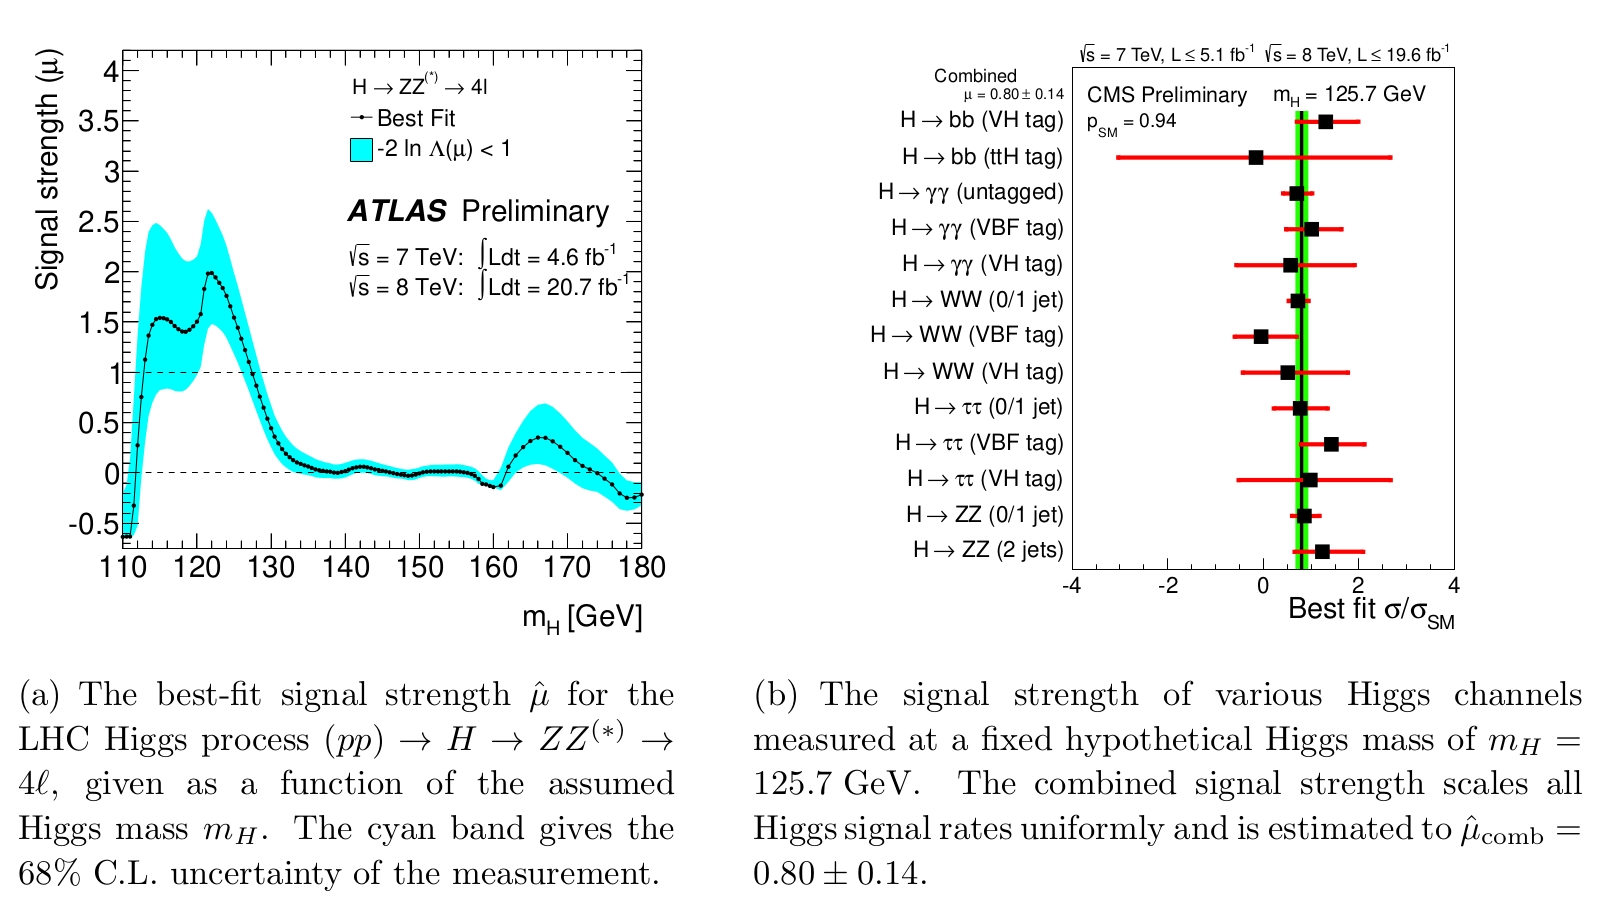
\includegraphics[scale=0.3]{images/signal1.jpg}
\caption{(a)signal strength modifiers by ATLAS \cite{<ss4>},
(b)the best fit rates according to CMS \cite{<ss3>}.}
\label{fig:sig1}
\end{figure}
The plot on the left (taken from \cite{<ss3>}) displays the measured signal strength modifier value, which is denoted by $\hat{\mu}$, in the interaction of $pp \rightarrow H\rightarrow ZZ^{\ast} \rightarrow 4l$ versus $m_H$ (black line) and an uncertainty $\pm1\sigma$ in measured rate is represented by the cyan band. Since the signal strength modifier illustrated in Fig.\ref{fig:sig1} (dashed line) is measured relative to its SM value ($\hat{\mu}$ = 1, it also encapsulates the theoretical uncertainties measured in branching ratios and cross section \cite{<ss4>}. The absence of signal-background interference in the signal model of SM never gives $\hat{\mu} < 0$, as seen in Fig.\ref{fig:sig1}, the measured value of $\hat{\mu}$ is permitted to have negative values. These negative values come from downwards statistical fluctuations in the data corresponding to the expected background value (the average expected background is $\hat{\mu}$ = 0).\\ 
To keep the authenticity intact, we retain full range of values of signal strength $\hat{\mu}$. In the following paragraph below we will see, the relevance of Higgs-Signals is restricted for range of masses in which the values $\hat{\mu}$ are detected. Hence accelerators should publish the mass regions where even SM Higgs signal are not measured.
The other example from CMS for Higgs-Signals input has been illustrated in the plot on right side of Fig.\ref{fig:sig1}(b) \cite{<ss4>}. Signal strength modifiers are summarized for Higgs decay modes at a value of $m_H$ = 125.7 GeV, where this value is commonly stated as it gives the maximum significance for a signal. It is essential to point out that when we fix a value for $m_H$, the plot also demonstrates different properties of various channels shown in Fig.\ref{fig:sig1}(b). Here, the horizontal error bars seen on $\hat{\mu}$ the measured values correlate the 1$\sigma$ uncertainties which are inclusive of SM, statistical and systematic uncertainties.\\
The Higgs-Signals matches the experimental signal strength modifier values with the predicted Higgs sector values in arbitrary models. The users give the predicted model for each parameter point to be tested over time known as simulations. We use five partonic subprocesses simulations for Higgs-Signals: gluon gluon fusion ($ggH$), vector boson fusion ($VBF$), vector boson associated production ($HW /HZ$), or top quark associated production ($ttH$) \cite{<ss5>}.\\
At base, Higgs-Signals runs on the LHC Higgs production cross sections and brancing ratios at centre-of-mass energy = 7 and 8 TeV as HiggsBounds-4, a tool which tests models of Higgs sectors having neutral and charged Higgs bosons, \cite{<ss3>}\cite{<ss5>}\cite{<ss6>}\cite{<ss7>}.\\
According to the theory, if signal strength modifier is predicted from one Higgs boson H, it is programmed in Higgs-Signals as
\begin{equation}
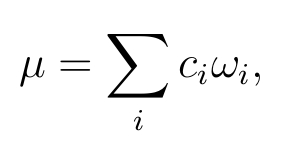
\includegraphics[scale=0.3]{images/hs1.jpg}
\end{equation}
here summation is over all the analysis channels used. A particular channel is specified by a distinct production and a distinct decay mode. Signal strength of a particular channel is defined as
\begin{equation}
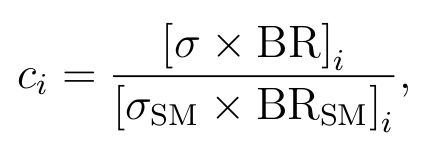
\includegraphics[scale=0.3]{images/hs2.jpg}
\end{equation}
and the SM channel weight as
\begin{equation}
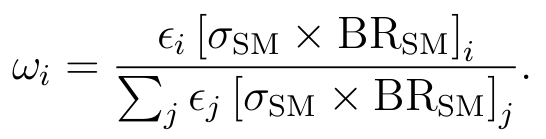
\includegraphics[scale=0.3]{images/hs3.jpg}
\end{equation}
The SM weights include the corresponding efficiencies, $\epsilon_{i}$ from the experiment, for the specific channels. If they are mentioned in experimental publications, we can use these numbers for Higgs-Signals, and have reliable comparison between the experimental data  and theory for specific channels. Where the efficiencies for channels are not known, all values are set to $\epsilon_{i}\equiv1$. Although many a times observable's close values for the channel efficiencies are calculated by reconstruction of fit results on scale factors of cross sections or coupling strengths in production.
As a caution it must be noted; if the model contains a non-standard tensor structure for the particles to be measured, which can be figured out from the data, the processes might include notable discrepancies in the kinematic distributions measured experimentally and in turn violate the signal efficiency acceptance in the data analyses of Higgs.
\section{Event Categorization}
\label{section:ec}
For the optimization of production modes of Higgs boson, signal events are divided into specific event categories. Categories are divided using observables typically from supplementary objects in the event, which have different sensitivity for different production modes. In Run I of LHC, two categories were defined using observed number of jets in an interaction, where fermion-Higgs and $V B \PHiggs$ couplings could already be measured. Run II of LHC had a more diversified categorization, which targets five main production mechanisms. Chosen signal events are divided into mutually exclusive event categories, each of which dominates a production mode.\\
This section will briefly review observable used in the categorization before stating the categorizations for 2016, 2017 and 2018 analysis, respectively.\\

\textbf{Categorizing Objects}\\
To acquire information about Higgs boson production mechanisms, apart from the four selected leptons, additional objects in the detector during each interaction are considered. Additional leptons which we describe as leptons that are not involved in selected $ZZ$ candidates and selected jets are taken into account. Event categorization has two types of input as observable: one which counts the number of additional objects in the event and the other which is the matrix-element based production discriminant based on jet kinematics and leptons.
\begin{enumerate}
    \item Selected jets number, for specific production mechanism such as $VBF, VH$ (1-2 jets in the event), and $\Ptop \Bar{\Ptop}\PHiggs$ (3 or more jets as in the event),
    \item Selected b-tagged jets number, which focuses on $ZH$ with $\PZ \rightarrow \Pqb \Paqb$ and $\Ptop \Bar{\Ptop}\PHiggs$,
    \item Additional leptons number, aiming at $\Ptop \Bar{\Ptop}\PHiggs\PHiggs$ and leptonic VH events,
    \item Opposite-sign same-flavour leptons pair number, which are unique for leptonic $\Ptop \Bar{\Ptop}\PHiggs$ and leptonic $ZH$ events.
    \item The observable which targets $VH$ events with neutrinos as decay products.
    \item Also the observable that counts the object numbers in an event, observable with neutrinos sensitivity and missing transverse momentum $E^{miss}_T$. 
\end{enumerate}

\subsection{2016 Data Categorization}
If an event does not fulfil requirements of selection for a particular category, it is considered for the subsequent category. In 2016 data accumulation at CMS experiment seven categories were selected:
\begin{SCfigure}
\centering
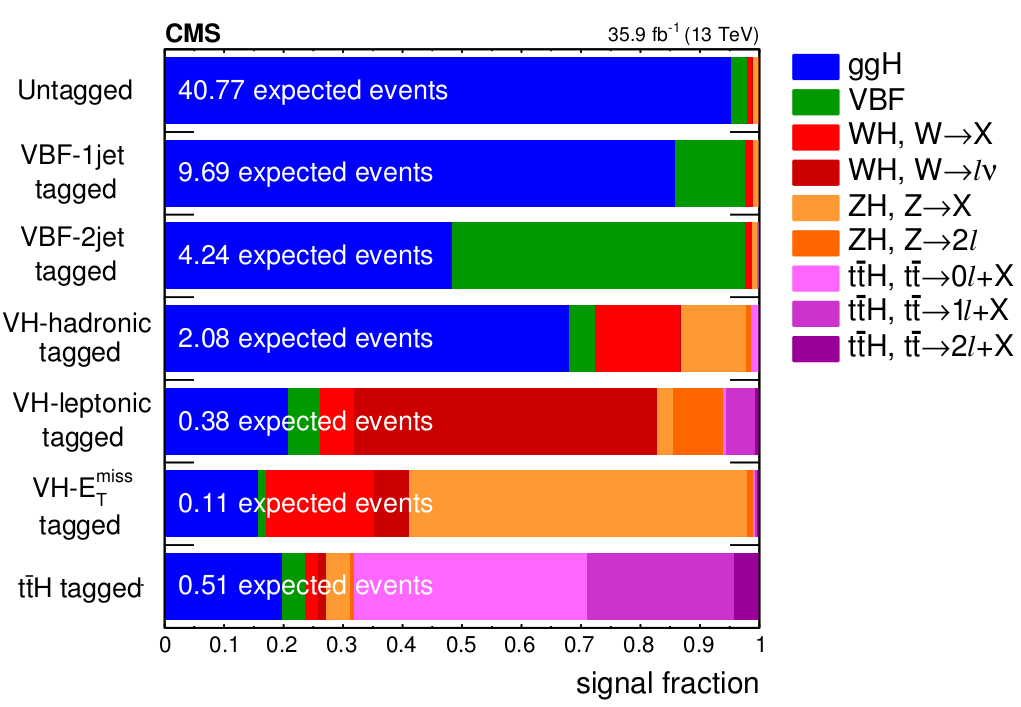
\includegraphics[scale=0.25]{images/cat1.png}
\caption{Composition of the categories in 2016 analysis in the $118 < m_{4l} < 130$ GeV window. The symbol X is for particles other than electrons muons.  \cite{<thesis>}.}
\label{fig:cat1}
\end{SCfigure}
\begin{itemize}
    \item \textbf{2jet-VBF} which has 4 leptons. 2-3 jets where one is b-tagged at the most, or (4 or more) not b-tagged jets. $D^{ME}_{VBF - 2j}> 0.5$.
    \item \textbf{hadraonic-VH} which has 4 leptons. 2-3 jets where one is b-tagged at the most, or (4 or more) not b-tagged jets. $D^{ME}_{VH} \equiv max(D^{ME}_{ZH}, D^{ME}_{WH}) > 0.5$.
    \item \textbf{leptonic-VH} should have 3 jets at minimum, exactly 1 additional lepton , 1 additional pair of OS, same-flavor leptons and no b-tagged jets. It can also contain events with at minimum 1 additional lepton and zero jets.
    \item \textbf{$\Ptop \Bar{\Ptop}\PHiggs$} should have at minimum 4 jets in which at minimum 1 is b-tagged, or at minimum 1 additional lepton.
    \item \textbf{$E^{miss}_{T}$-VH} should have 4 leptons, at most 1 jet and $E_{T}^{miss}$ greater than 100 GeV.
    \item \textbf{1jet-VBF} should have 4 leptons, exactly 1 jet and $D^{ME}_{VBF - 1j} > 0.5$.
    \item The \textbf{Untagged} entails the rest of selected events.
\end{itemize}
\vspace{4mm}
\subsection{2017 Data Categorization}
The 2017 data analysis was to be preliminary done by promptly reproduced data and the $E^{miss}_{T}-VH$-tagged category was dropped and another one in its place was adopted for the 2017 event categorization. The following seven categories are considered:
\begin{itemize}
      \item \textbf{2jet-VBF} which has 4 leptons. 2-3 jets where one is b-tagged at the most, or (4 or more) not b-tagged jets. $D^{ME}_{VBF - 2j}> 0.5$.
    \item \textbf{hadraonic-VH} which has 4 leptons. 2-3 jets where one is b-tagged at the most, or (4 or more) not b-tagged jets. $D^{ME}_{VH} \equiv max(D^{ME}_{ZH}, D^{ME}_{WH}) > 0.5$.
    \item \textbf{leptonic-VH} should have 3 jets at minimum, exactly one additional lepton , one additional pair of OS, same-flavor leptons and no b-tagged jets. It can also contain events with at minimum 1 additional lepton and zero jets.
    \item The \textbf{hadronic-$\Pqt\Paqt\PHiggs$} should have 4 jets at minimum, of which at least 1 is b-tagged and there are no additional leptons.
    \item The \textbf{leptonic-$\Pqt\Paqt\PHiggs$} should have 1 additional lepton.
     \item \textbf{1jet-VBF} should have 4 leptons, exactly 1 jet and $D^{ME}_{VBF - 1j} > 0.5$.
    \item The \textbf{Untagged} entails the rest of selected events.
\end{itemize}
\begin{figure}[h]
\centering
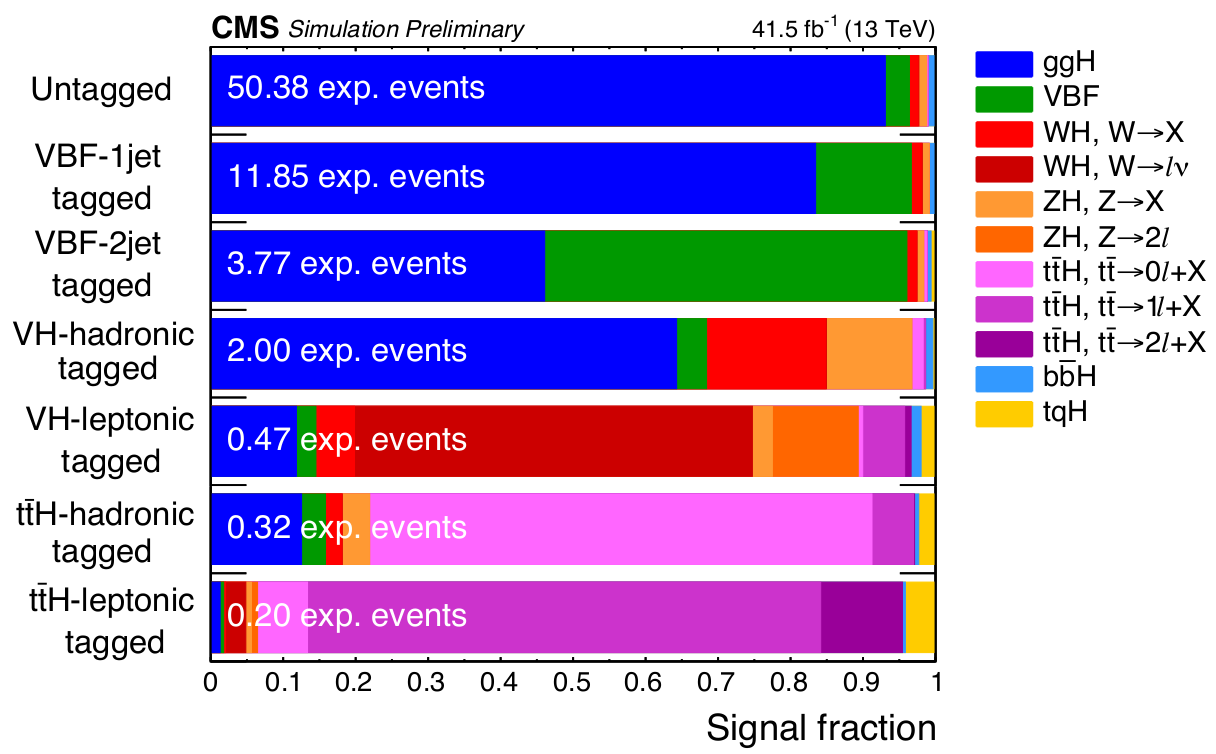
\includegraphics[scale=0.25]{images/cat2.png}
\caption{Event categories of the 2017 data analysis in the $118 < m_{4l} < 130$ GeV window. The X symbol stands for particles other than electrons muons.\cite{<thesis>}}
\label{fig:cat2}
\end{figure}

\subsection{2018 Data Categorization}
In 2018 categorization a VH-MET Category is added along with 2017 reconstructed events and categories are further split into sub categories.
\begin{itemize}
    \item The \textbf{VH-MET} requires one missing lepton at the vmost, no more than 1 jet and and missing transverse momentum $E^{miss}_{T}> 100$ GeV.
\end{itemize}
Reconstructed events are further subdivided in the next step of the categorization, the Untagged,  VBF-2jet, VH-leptonic, and VH-hadronic categories are then divided further, exploiting additional variables e.g. the transverse momentum of the ZZ candidate and the invariant mass of the two leading jets as illustrated in Fig.\ref{fig:cat3}. The number of event categories used each year corresponding to their integrated luminosity are mentioned in Table.\ref{tab:dat}.

\begin{figure}
\centering
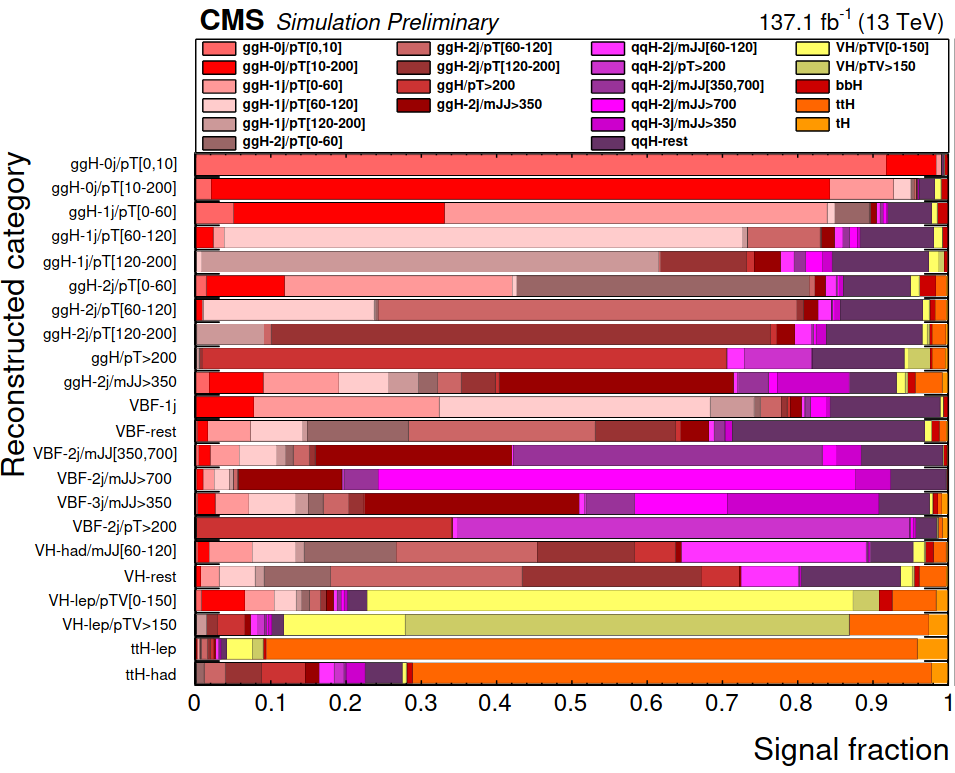
\includegraphics[scale=0.26]{images/cat3.png}
\caption{Distributions after event reconstruction for the mass range $105 < m_{4l} <140$ GeV in year 2018.\cite{<2021>}}
\label{fig:cat3}
\end{figure}
\begin{table}[]
    \centering
    \begin{tabular}{|c|c|c|}
    \hline
       Data Year  & Integrated Luminosity & Event Categories \\
      \hline
      2016 & 35.9 fb$^{-1}$ & 6 \\
    2017 & 41.5 fb$^{-1}$ & 7 \\
    2018 & 59.7 fb$^{-1}$ & 8 \\
    \hline
    \end{tabular}
    \caption{Analysis Factors}
    \label{tab:dat}
\end{table}


\section{Analytical Techniques}
After defining $H \rightarrow ZZ^* \rightarrow 4l$ analysis building blocks (event categories), the most integral part is to verify how the final measurements are in accord with the simulations. During the Run I of LHC, the search for Higgs boson was at forefront, by searching for specific events in an unlimited amount of events in accordance with the Standard Model prediction and organizing it. The Run II shifted the focus to property measurements of Higgs and in looking for new physics. For modelling different properties, different statistical methods are used, and this section will introduce the statistical distributions used for model fitting.
\subsection{Gaussian Distribution}
\label{section:gd}
The Gaussian (Normal) PDF of $x$, a continuous random variable with $- \infty < x < \infty$ is described as,
\begin{equation}
    f (x; \mu \sigma^2) = \frac{1}{2 \pi \sigma^2} exp \left ( \frac{-(x-\mu)^2}{2 \sigma^2} \right),
\end{equation}
where $\mu$ is the mean and $\sigma^2$ is the variance of Gaussian distribution. They are given as,
\begin{equation}
    \begin{aligned}
        &E[x] = \int ^{\infty}_{- \infty} x \frac{1}{2 \pi \sigma^2} exp \left ( \frac{-(x-\mu)^2}{2 \sigma^2} \right)dx = \mu, \\
        &V[x] = \int ^{\infty}_{- \infty} (x-\mu)^2 \frac{1}{2 \pi \sigma^2} exp \left ( \frac{-(x-\mu)^2}{2 \sigma^2} \right)dx = \sigma^2
    \end{aligned}
\end{equation}
$E[x]$ gives a range of values where $x$ are likely to be detected. For instance, the $f(x)$ might show two widely separated peaks, where $E[x]$ is in the middle and $x$ occasionally (or is never) observed. The variance $V[x]$ represents the spread in data given by $x$, around the mean value.
\begin{figure}[h]
\centering
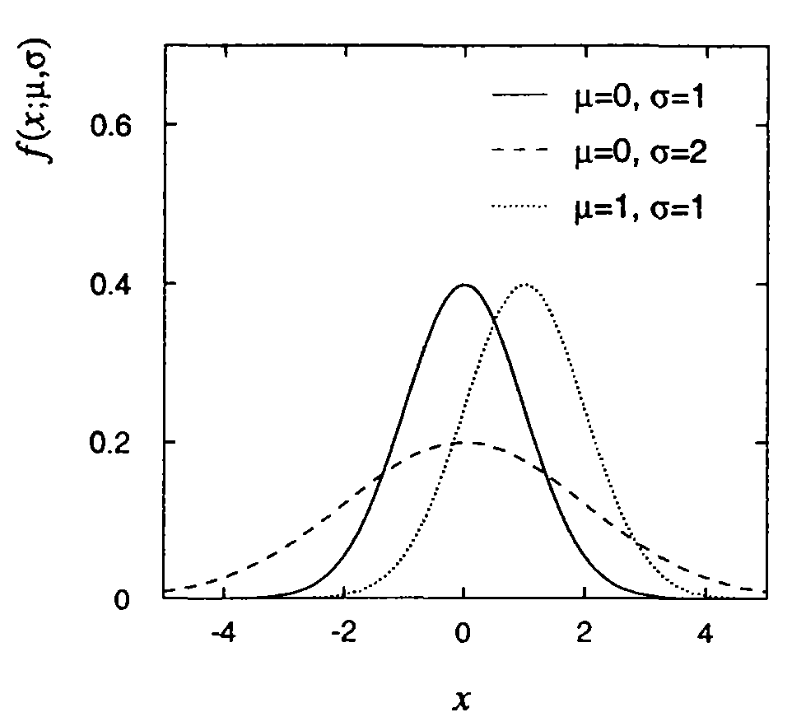
\includegraphics[width=0.3\textwidth]{images/var.png}
\caption{The Gaussian PDF for various values of the parameters $\mu$ and               $\sigma$.}
\label{fig:var}
\end{figure}
In a particular case, the standard Gaussian $\phi(x)$ (with $\mu = 0$ and $\sigma=1$ is defined as such, 
\begin{equation}
    \phi(x) = \frac{1}{\sqrt{2 \pi}} exp ( - x^2/2), 
\end{equation}
with $\Phi(x)$ as corresponding distribution.
\begin{equation}
    \Phi(x) = \int ^x_{- \infty} \phi(x)' dx'.
\end{equation}
To check if $y$ is distributed according to a Gaussian PDF, then
\begin{equation}
x= \frac{y-\mu}{\sigma}
\end{equation}
here the cumulative distributions are correlated by $F(y) = \Phi(x)$. There is no analytical representation of cumulative distribution, so we have to perform numerical evaluation. Values of $\Phi(x)$ along with $x_0 = \Phi(x)^{-1}(\alpha)$ are tabulated in reference books \cite{<gd1>,<gd2>,<gd3>,<gd4>} and instilled in computer program libraries, e.g. the routines FREQ and GAUSIN \cite{<gd5>}. The central limit theorem gives significance to Gaussian distributions. The theorem states that the sum of n random continuous independent variables $x_i$ having mean value $\mu_i$ with variance $\sigma_i$ becomes a Gaussian random variable when the limit n approaches to infinity, having mean value $\mu = \sum^n _{i=1} \mu_i$ and variance $\sigma^2 = \sum^n _{i=1} \sigma_i^2$. This provides measurement errors with Gaussian random variables treatment, and is extended till the total error becomes the sum of unlimited values giving small contributions from each variable.\\
The N-dimensional generalization of the Gaussian distribution is  defined by 
\begin{equation}
    f(x; u,V) = \frac{1}{(2 \pi)^{N/2}|V|^{1/2}}exp \left[- \frac{1}{2}(x-\mu)^T V^{-1}(x-\mu)\right],
\end{equation}
here column vectors are given by $x$ and $\mu$, and row vectors by $x^T$ and $\mu^T$ and $|V|$ represents the determinant of a symmetric $N \times N$ matrix $V$, with free parameters amounting to $N (N + 1) /2$. The (co)variances and expectation values are;
\begin{equation}
    \begin{aligned}
        E[x_i]=\mu_i\\
        V[x_i]=V_{ii}\\
        cov[x_i, x_j]=V_{ij}.
    \end{aligned}
\end{equation}
\subsection{Landau Distribution}
\label{section:ld}
In nuclear and particle physics there is mostly energy loss $\triangle$ when a charged particle travels through a layer of matter with a known thickness, which is given with the probability density $f (\triangle;\beta)$. Landau \cite{<LD>}, was the first one to derive this probability density given by,
\begin{equation}
    f(\triangle;\beta) = \frac{1}{\xi} \phi (\lambda), \hspace{3mm} 0 \leq \triangle < \infty,
\end{equation}
here the parameter $\xi$ and $\lambda$ relate to the property of the material, $\beta = v/c$ to the velocity of the particle, and $\phi (\lambda)$ is the PDF of the dimensionless random variable $\lambda$. These quantities are given by
\begin{equation}
    \begin{aligned}
    &\xi = \frac{2 \pi N_A e^4 z^2 \rho \sum Z}{m_e c^2 \sum A}\frac{d}{\beta^2},\\
    & \lambda = \frac{1}{\xi} \left [\triangle - \xi \left(log \frac{\xi}{\epsilon'}+1- \gamma_E \right) \right],\\
    &\epsilon' = \frac{I^2 exp (\beta^2)}{2 m_e c^2 \beta^2 \gamma^2},
    \end{aligned}
\end{equation}

where $N_A$ is the Avagadaro's number, $m$, $e$ are mass and charge of the electron, $z$ is incident particle's charge, $\sum Z, \sum A$, gives summation over the atomic number and atomic weights of the molecular substance, $\rho$ is density, $d$ is thickness, $I=I_0 Z$ where $I_0$ = 13.5eV is the ionization characterisation of the material, $\gamma = \sqrt{1-1/\beta^2}$, and Euler's constant $\gamma_E = 0.5772 \cdots$. The function: 
\begin{equation}
\begin{aligned}
    &\phi(\lambda)= \frac{1}{2 \pi i} \int^{\epsilon + i \infty}_{\epsilon - i \infty} exp(u log u + \lambda u)du,\\
    &\phi(\lambda)= \frac{1}{\pi} \int^{\infty}_{0} exp(- u log u + \lambda u) sin \pi u du,
    \end{aligned}
\end{equation}
\begin{figure}[h]
     \centering
     \begin{subfigure}[b]{0.45\textwidth}
         \centering
         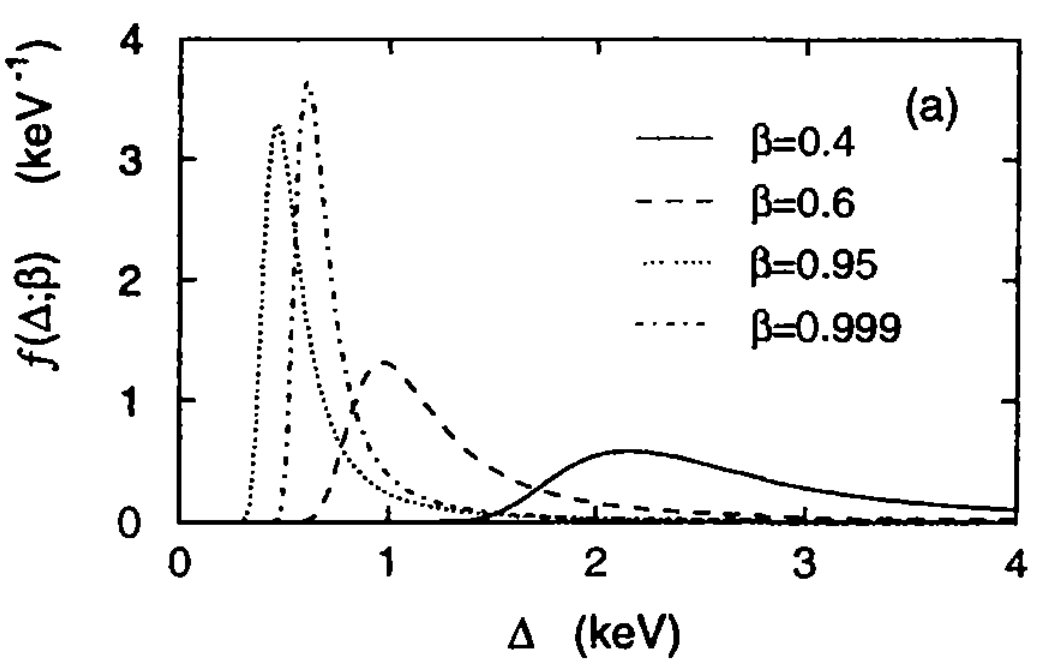
\includegraphics[width=\textwidth]{images/LD2.png}
     \end{subfigure}
     \hfill
     \begin{subfigure}[b]{0.45\textwidth}
         \centering
         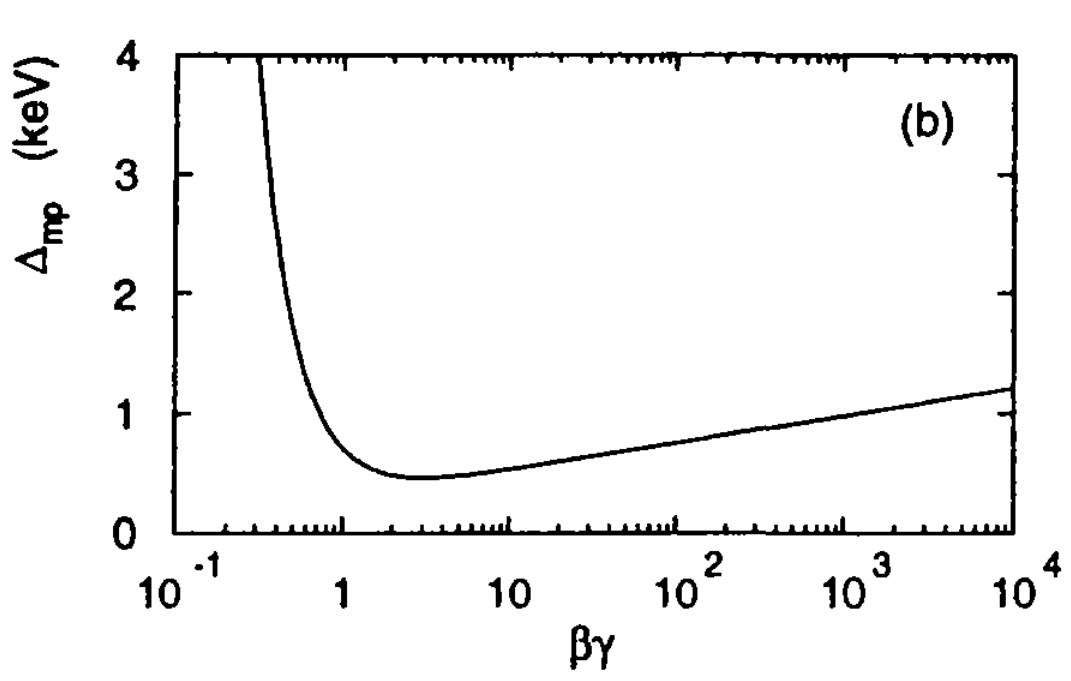
\includegraphics[width=\textwidth]{images/LD.png}
     \end{subfigure}
     \hfill
        \caption{(a)The Landau probability density with energy loss $\triangle$ of a charged particle travelling through a 4 mm thick layer of argon gas at stp at different values of the velocity $\beta$. (b)The peak modes in (a) as a function of $\beta_\gamma$ from Eq.3.14}
        \label{fig:LD}
\end{figure}
The distribution of energy loss is demonstrated in Fig.\ref{fig:LD}(a) for different $\beta$ values. There are no mean and higher moments of the Landau distribution because of long tail extending to high values of $\triangle$, i.e. the integral $\int^{\infty}_{0} \triangle^n f(\triangle) d\triangle$ diverges for $n\ge1$. The Fig.\ref{fig:LD}(b) demonstrates that the common mode $\triangle_{mp}$ is sensitive to the particle's velocity which was numerically computed \cite{<mac69>} to be, 
\begin{equation}
    \triangle_{mp} = \xi [log(\xi/\epsilon')+0.198],
\end{equation} 
The `Bethe-Bloch formula' as the above equation is popularly known as and given in books e.g. Subatomic Physics by Henley \cite{<sap>}, is basis on which charged particles are identified by measurement of ionization energy loss \cite{<bbf>}.\\
As for Landau, the mean and higher moments do not exist for the Breit-Wigner distributions, this is due to the fact that probability densities which are used to describe physical processes require finite moments. When measuring energy loss $\triangle$ of a particle repetitively, the average would converge to some value, as energy loss can never be higher than the energy of the incoming particle. Same is the case for the mass of a resonance particle, it should never be less than the sum of the rest masses of corresponding decay products, and higher than the center-of-mass energy of the reaction where it occurred. This creates a problem when the Cauchy and Landau distributions are approximating models of physical system but break down at the tails, which in the PDF causes the mean and higher moments to diverge \cite{<cowan>}.
\subsection{Breit-Wigner Distribution}
\label{section:bwd}
The Cauchy or Breit-Wigner probability density function of the continuous variable $x$ $(- \infty < x < \infty)$ is defined as, 
\begin{equation}
    f(x) = \frac{1}{\pi} \cdot \frac{1}{1 + x^2}.
\end{equation}
Given below is a special case of the Breit-Wigner distribution we see in particle physics,
\begin{equation}
    f (x; \Gamma, x_0) = \frac{1}{\pi} \frac{\Gamma/2}{\Gamma^2 /4  + (x- x_0)^2},
\end{equation}
where the mass is given as $x_0$ and width as $\Gamma$ of a resonance particle as illustrated in Fig.\ref{fig:bw}; $x_{0}$ represents the peak mode and $\Gamma$ represents the full-width of the peak at half of the maximum height \cite{<gd3>,<bwd>}.\\
\begin{SCfigure}[][h]
    \centering
    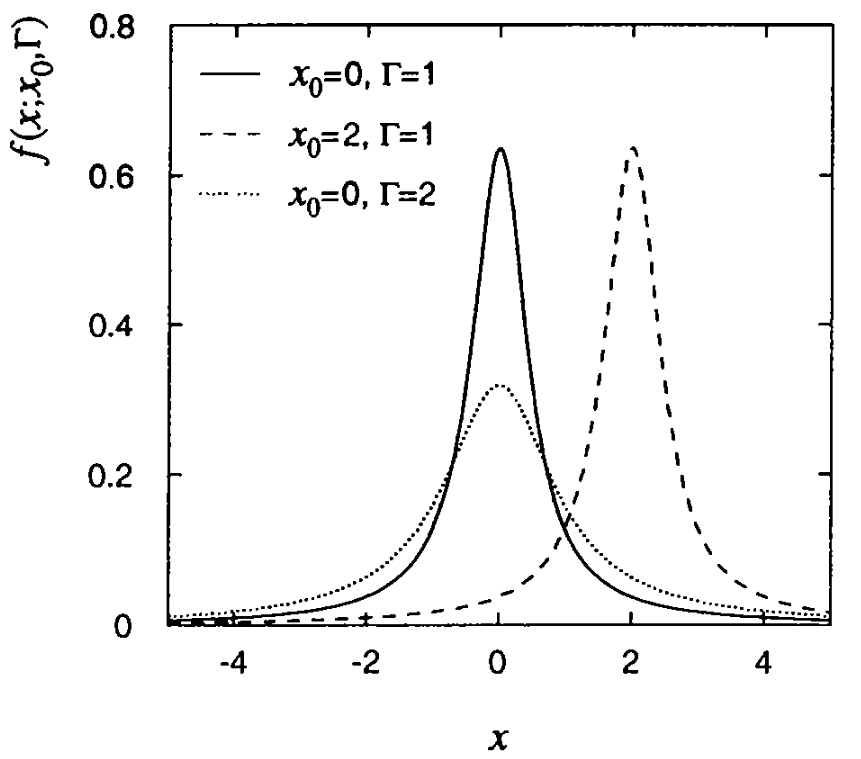
\includegraphics[scale=0.2]{images/bw.png}
    \caption{The Cauchy (Breit-Wigner) PDF for different values of the parameters $x_0$ and $\Gamma$.}
    \label{fig:bw}
\end{SCfigure}
The Cauchy distribution does not have well defined expectation value, even with a symmetric PDF about zero (or $x_0$ for Eq.3.8). The integrals $\int^{0}_{-\infty} xf(x)dx$ and $\int^{\infty}_{0} xf(x)dx$ diverge separately on their own, along with variance and higher moments \cite{<cowan>}. The Cauchy distribution is a normal ratio distribution, a ratio of two normalised distributions with mean zero. For two random variables $p$ and $q$, the ratio distribution of a third random variable $w$ is defined as $w = p/q$. 
\subsection{Double Shouldered Crystal Ball Function}
\label{section:dcb}
The Crystal Ball function, named after the Crystal Ball (hermetic particle detector), is a PDF typically used when modelling various particle physics processes which have energy losses. It contains a Gaussian core portion shown in Fig.\ref{fig:gbw} and below a distinct threshold a power law end tail shown in Fig.\ref{fig:CBF}. It is a continuous function with continuous first derivatives. A Double Crystal Ball (DCB) Function has two power-law end-tails on both sides:
\begin{figure}[h]
    \centering
    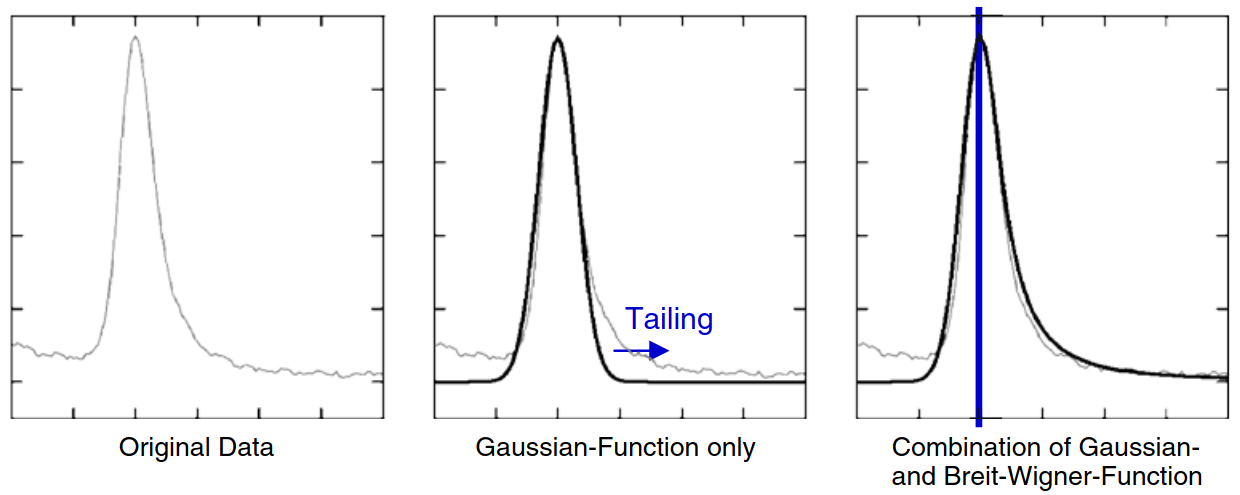
\includegraphics[scale=0.3]{images/gbw.png}
    \caption{A single spectrum of data, the application of the Gaussian function with a tail and the combination of Gaussian and Breit-Wigner-Function for best fit.}
    \label{fig:gbw}
\end{figure}
\begin{equation}
    dCB(\epsilon) = N \cdot 
    \left \{\begin{aligned} & D_1. (D_2 + |\epsilon|)^{-n_L}, \hspace{2mm} \epsilon < \alpha_L \\ &D_1 . (D_2+ |\epsilon|)^{-n_R}, \hspace{2mm} \epsilon > \alpha_R \\ &exp(- \epsilon^2/2),\hspace{1mm} \alpha_L \leq \epsilon \leq \alpha_R  \end{aligned} \right \} 
    \label{eqn:dcb}
\end{equation}
here $\epsilon = (m_{4l} - m_H - \triangle m_H )/ \sigma_m$. DCB with 6 independent parameters, captures the Gaussian core $(\sigma_m)$ of mass resolution function of the four leptons and $\triangle m_H$ mass shift of the peak, and the left- and right-hand tails originating from tracker bremsstrahlung emitted by leptons, which exist for both electrons and muons, and from the non-Gaussian mis-measurements which are unique for events of electrons with the experimental material. The effectiveness of the side tails is shown by the power $n_L , n_R$, respectively. Here parameters $\alpha_L , \alpha_R$ define slicing of the tails and $\sigma_m$ defines the core. Parameters $D_1$ and $D_2$ are not independent; they are described by function continuity along with it's first derivatives. N is the normalizing constant.\cite{<toni>}
\begin{figure}
    \centering
    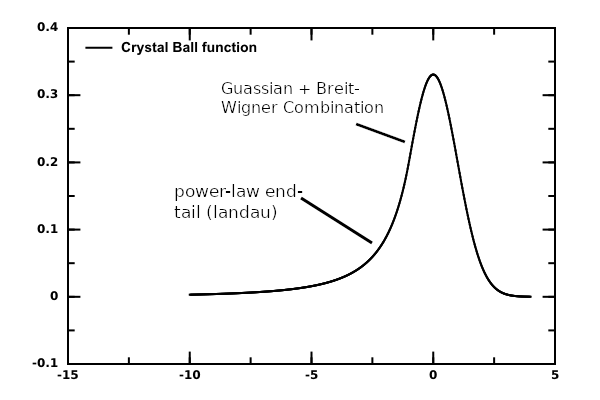
\includegraphics[scale=0.4]{images/CBF.png}
    \caption{Double Crystal Ball Function}
    \label{fig:CBF} 
\end{figure}
\subsection{Pull Distribution}
\label{section:pd}
The pull of a bin is defined as the difference between model function and value of the histogram, divided by the error of the histogram value $(\frac{residue}{error})$. If the model describes the histogram, the pulls should be distributed as a normal distribution with a width of 1 centered around the origin, i.e. plot of the distribution $\Phi_i$ should be a Gaussian, centered at 0, and width=1.
\begin{figure}[h]
    \centering
    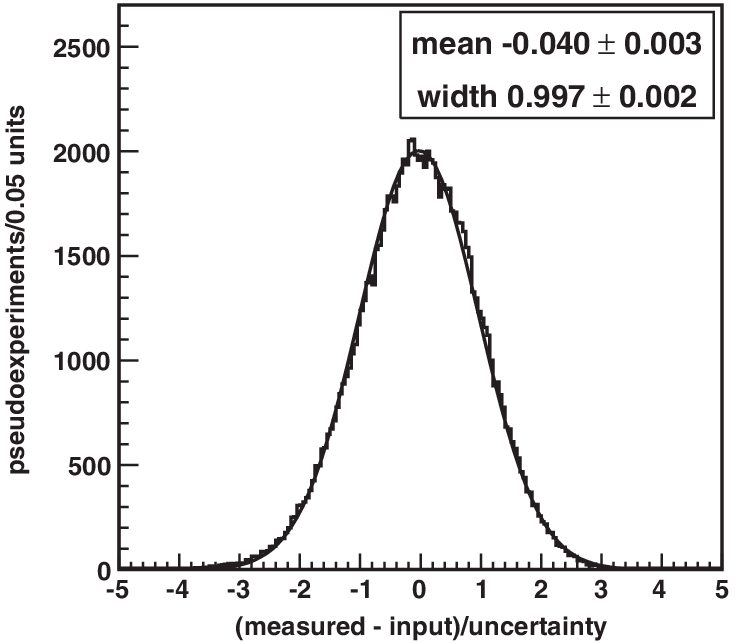
\includegraphics[scale=0.25]{images/pd.png}
    \caption{Pull distribution from pseudo-experiments run with the likelihood used to find the combined cross section \cite{<pd2>}.}
    \label{fig:pd}
\end{figure}
This controls the quality of the fit. If this test fails, we say that the used model does not match the experimental measurements, the measurements used for the weights are biased or error estimates are not properly estimated \cite{<pd1>}. Pull or stretch values of fitted parameter $i$ is defined as
\begin{equation}
    \triangle_i = (x_i - \mu)/ \sigma_i
\end{equation}
An example of pull distribution is given in Fig.\ref{fig:pd}. Some properties taken into account while plotting a pull are:
\begin{itemize}
    \item If not centered in $0 \rightarrow$ bias in measurement,
    \item If pull width $ < 1$, uncertainty is under-covered,
    \item If pull width $ > 1$, uncertainty is overestimated. 
\end{itemize}

\subsection{Chebyshev Polynomials}
\label{section:cp}
This relates to deriving a simple polynomial function $f(x)$ to fit to a given function  $g(x)$, that can be used to approximate the original function. This is especially useful when the original function is difficult to differentiate or integrate.
\clearpage
\textbf{Chebyshev Theorem}\\
\begin{wrapfigure}[]{l}{0.4\textwidth}
\vspace{-30pt}
\begin{center}
    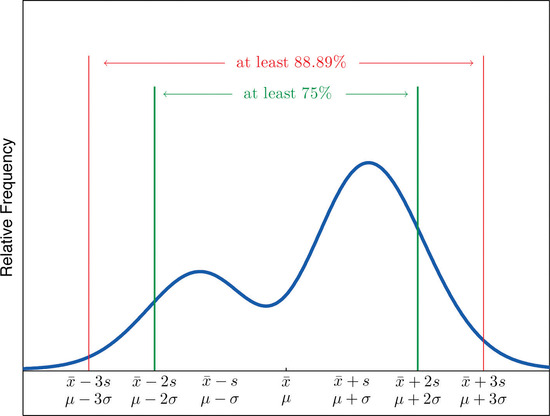
\includegraphics[scale=1]{images/CT.jpg}
\end{center}
\vspace{-20pt}
\caption{Chebyshev's Theorem \cite{<cheb1>}}
    \label{fig:ct}
    \end{wrapfigure}
    For any numerical data set as shown in Fig.\ref{fig:ct}:\\
\begin{enumerate}
    \item at least $1 - 1/\kappa^{2}$ events are inside $\kappa$ standard deviations of the mean, i.e. endpoints $\bar{x} \pm \kappa s $ for samples and endpoints $\mu \pm \kappa \sigma$ for populations where $\kappa > 1 $;
\end{enumerate}
For values only in $\xi \hspace{2mm} \epsilon \hspace{2mm}[1,-1]$ interval, the $x^{th}$ \textbf{Chebyshev's Polynomial} $T_x (\xi)$ is described as,
\begin{equation}
    T_x (\xi) \equiv cos (x\cdot arccos(\xi)), x=1,2, \cdots.
\end{equation}
This describes the function domain $arccos(x)$. First we consider the first three Chebyshev's polynomial and check if they are indeed polynomials;
\begin{equation}
    \begin{split}
        &T_I (\xi) = cos (0 arccos(\xi))=1,\\
        &T_{II} (\xi) = cos (1 arccos(\xi))=\xi,\\
        &T_{III} (\xi) = cos (2 arccos(\xi))=2 [cos(arccos(\xi))]^{2}-1=2 \xi^2 - 1,
    \end{split}
\end{equation}
Using the formula for double angle, $cos2\theta = 2 \cdot cos^2 \theta - 1$ to derive $T_{II}(\xi)$ and $cos(\alpha)+cos(\beta)= 2 cos(\frac{\alpha+\beta}{2})+cos(\frac{\alpha-\beta}{2})$ we derive the higher order polynomials. i.e.
\begin{equation}
    \begin{split}
        &\hspace{-15mm}T_{x+1}(\xi)+T_{x−1}(\xi)=cos[(x + 1)arccos(\xi)]+cos[(x−1)arccos(\xi)]\\
        & = cos [x\cdot arccos(\xi) + arccos(\xi)] + cos[x\cdot arccos(\xi) - arccos(\xi)]\\
        & =2 cos[x\cdot arccos(\xi)] cos [arccos(\xi)]\\
        & =2\xi T_x (\xi).
    \end{split}
\end{equation}
The Chebyshev polynomials uses recurrence relation,
\begin{equation}
    T_{x+1}(\xi) = 2\xi T_x(\xi) - T_{x - 1}(\xi), \hspace{2mm}  x=1,2, \cdots.
\end{equation}
This method shows that if we have a N degree Chebyshev's polynomial $T_N (x)$, $x$ has even(odd) powers corresponding to if N is even(odd). The first eighth terms in power series form and in Chebyshev's series form, are displayed in Table.\ref{tab:cp}.
\begin{table}
    \centering
    \begin{tabular}{c}
       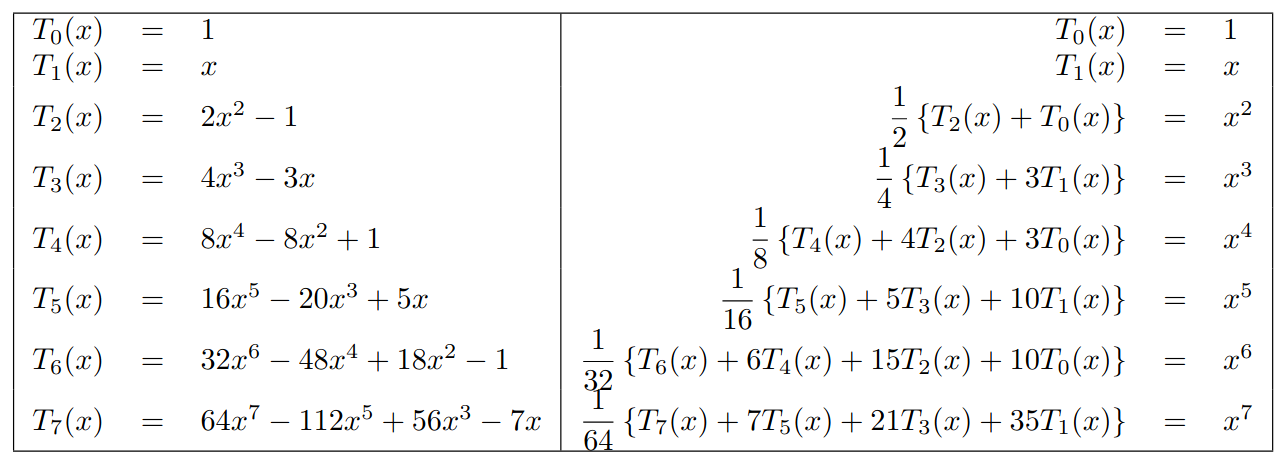
\includegraphics[scale=0.3]{images/cheb1.png} 
    \end{tabular}
    \caption{Chebyshev's Polynomial Conversion Table}
    \label{tab:cp}
\end{table}
The advantage of choosing Chebyshev's polynomial, shown in Fig.\ref{fig:cp2} $T_x(\xi)=cos(x arccos(\xi))$ as opposed to the power term $\xi^x$ for showcasing data for values $\xi_\epsilon$ $[ - 1,+ 1]$ is that $T_x(\xi)$ oscillates x number of times in between $\xi=-1$ and $\xi= + 1$. Also, with the increase in x value the end zero crossings on both side of data for $T_x(\xi)$ almost nears, but never cross, the range endpoints $\xi =-1$ and  $\xi = + 1$. Hence, the polynomials of Chebyshev provide precise estimation for distributions described in the range $[- 1, + 1]$ with better shape characterization than the power series form \cite{<cheb2>}.\\
\begin{figure}
    \centering
    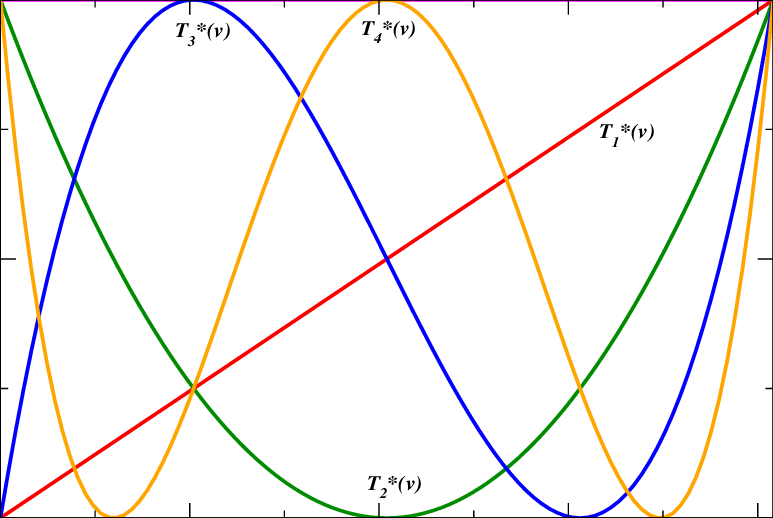
\includegraphics[scale=0.2]{images/cheb2.png}
    \caption{Chebyshev First 4 Polynomials }
    \label{fig:cp2}
\end{figure}


\textbf{Recommendations for Fitting Data}
\begin{enumerate}
    \item  Use the lowest order polynomial that gives a reasonable approximation to the data.  Do not over fit the data, or the fitted polynomial will follow every bit of the noise on the data.
    \item Realise that the fit may be bad near the ends of the data. 
    \item  Do not use the polynomial approximation outside the range of the input data. i.e. Do not extrapolate the data!
\end{enumerate}